
 % ********** Rozdział 3 **********

\chapter{Opis projektu}
\section{Opis struktury projektu}

\subsection{Diagram klas}


\begin{figure}[H] % Użyto opcji H
    \centering
    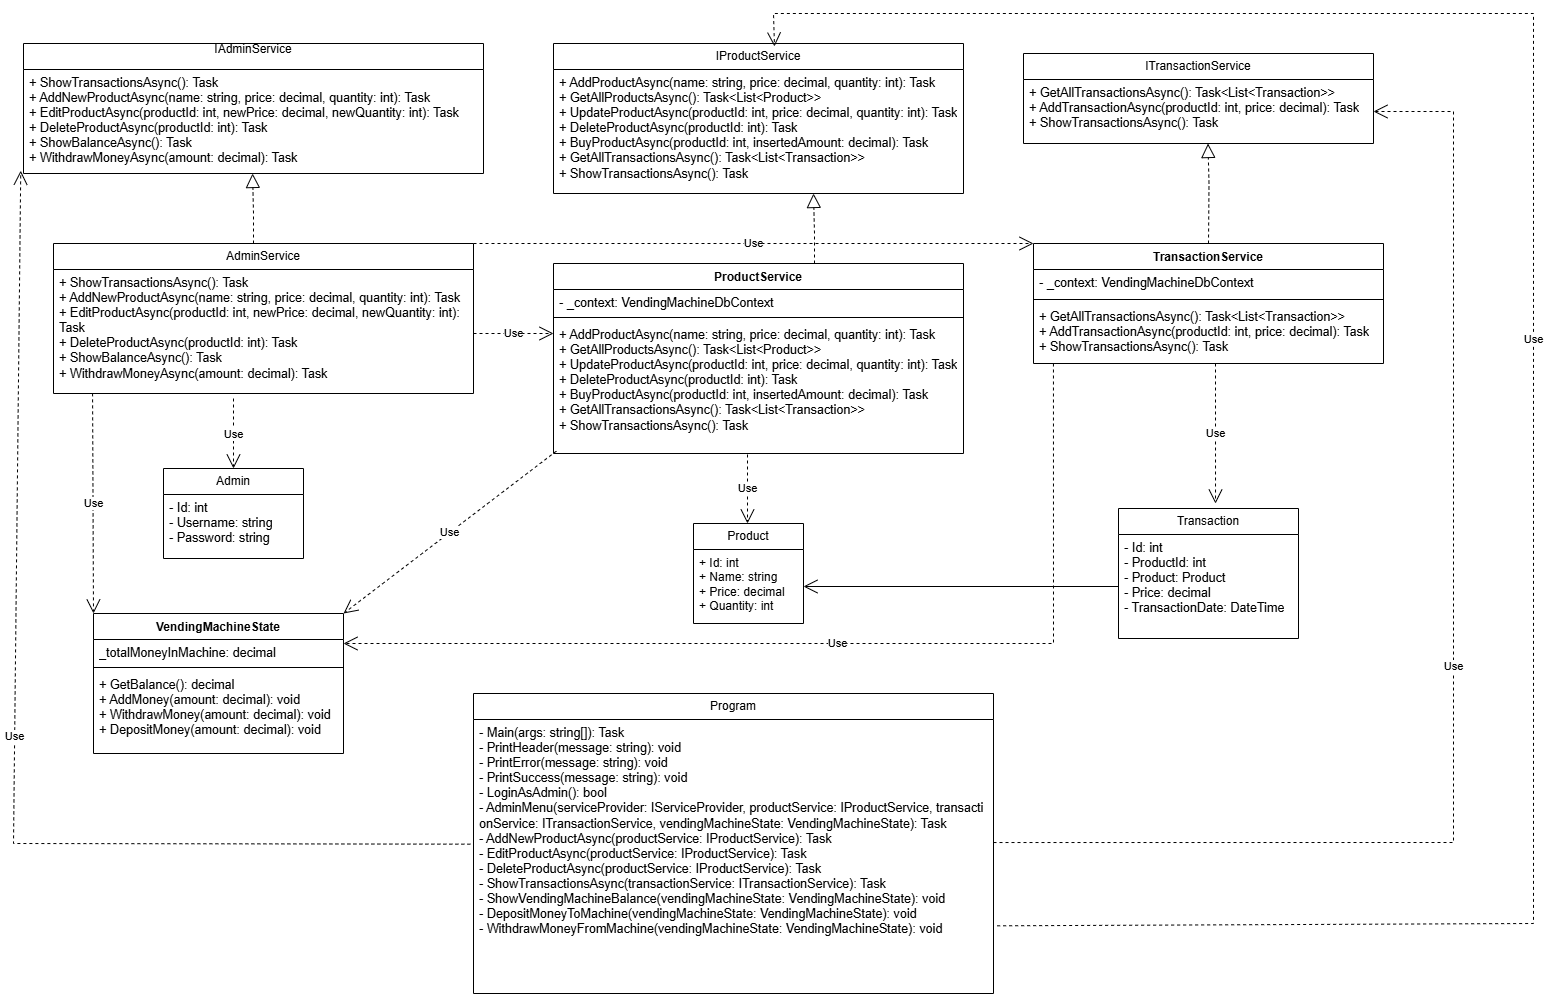
\includegraphics[width=1\textwidth ]{grafiki/diag_klas.PNG}
    \caption{\footnotesize Diagram przedstawiający strukturę klas programu}	
\end{figure}
\newpage

\subsection{Struktura diagramu klas}

Struktura diagramu klas przedstawia zależności między klasami, ich funkcje oraz relacje. Każda klasa ma określoną rolę w symulacji działania automatu z napojami i współpracuje z innymi klasami, aby zapewnić kompleksowe doświadczenie użytkownika, zarządzanie zapasami, obsługę transakcji oraz administrowanie stanem automatu.

\subsubsection*{Program}
Klasa główna aplikacji, która zarządza działaniem całego systemu. Odpowiada za uruchomienie aplikacji, obsługę interakcji użytkownika, takich jak wybór opcji z menu, zakupy, zarządzanie stanem automatu i wyświetlanie komunikatów. Korzysta z różnych serwisów, takich jak AdminService, TransactionService i ProductService, aby zapewnić poprawne działanie aplikacji.

\subsubsection*{AdminService}
Klasa zarządzająca administracyjnymi funkcjami aplikacji. Odpowiada za zarządzanie zapasami produktów w automacie, aktualizowanie stanów produktów, sprawdzanie dostępności towarów oraz monitorowanie transakcji. AdminService komunikuje się z klasami ProductService i TransactionService w celu zarządzania zapasami i obsługi transakcji. Ponadto korzysta z klasy VendingMachineState do monitorowania stanu maszyny.

\subsubsection*{TransactionService}
Klasa odpowiedzialna za obsługę transakcji w aplikacji. Zajmuje się realizowaniem zakupów, obliczaniem wydawanej reszty oraz zapisami transakcji. TransactionService współpracuje z klasą ProductService w celu obliczania kosztów produktów i aktualizowania zapasów, oraz z klasą Transaction w celu rejestrowania szczegółów transakcji.

\subsubsection*{ProductService}
Klasa odpowiedzialna za zarządzanie produktami w automacie vendingowym. Umożliwia dodawanie nowych produktów, usuwanie ich, edytowanie cen i dostępnych ilości. ProductService współpracuje z AdminService, aby zapewnić aktualizację zapasów w automacie i umożliwia przechowywanie informacji o produktach w bazie danych.

\subsubsection*{VendingMachineState}
Zarządza stanem maszyny, takim jak dostępne monety, zapasy produktów i ogólny stan operacyjny. Wykorzystywana przez AdminService i TransactionService.

\subsubsection*{Transaction}
Klasa reprezentująca pojedynczą transakcję w systemie. Zawiera informacje o dokonanym zakupie, takich jak zakupiony produkt, jego cena, kwota zapłacona przez klienta, reszta oraz status transakcji. Transaction jest używana przez TransactionService do przechowywania szczegółów transakcji oraz współpracuje z Product w celu aktualizacji zapasów po dokonaniu zakupu.

\subsubsection*{Product}
Klasa reprezentująca pojedynczy produkt w automacie vendingowym. Zawiera dane dotyczące produktu, takie jak jego nazwa, cena, ilość w zapasie i unikalny identyfikator. Product jest używana przez ProductService do zarządzania informacjami o produktach oraz przez TransactionService do obliczania kosztów produktów w transakcjach.



\section{Opis techniczny projektu}


\subsection{Język programowania:}
Projekt został zaimplementowany w języku C\# .NET 7.0 (Console App).

\subsection{Narzędzia:}
\begin{itemize}
    \item Środowisko programistyczne: Projekt był rozwijany w środowisku Visual Studio, które zapewnia wsparcie dla tworzenia aplikacji w języku C\# oraz ułatwia zarządzanie projektem.
    \item Baza danych: Aplikacja korzysta z SQL Server jako systemu zarządzania bazą danych, a do komunikacji z bazą użyto Entity Framework Core, zapewniając prostą integrację danych
\end{itemize}

\subsection{Minimalne wymagania sprzętowe:}
Minimalne wymagania sprzętowe dla uruchomienia aplikacji zależą głównie od zasobów potrzebnych do uruchomienia systemu operacyjnego oraz środowiska uruchomieniowego (.NET 7.0). Zazwyczaj są to:
\begin{itemize}
    \item Procesor: 1 GHz lub szybszy procesor (x86- lub x64-bitowy)
    \item Pamięć RAM: 1 GB dla systemów 32-bitowych lub 2 GB dla systemów 64-bitowych
    \item Dysk twardy: Minimum 5-10 MB wolnego miejsca na dysku twardym
    \item System operacyjny: Windows 7 lub nowszy
\end{itemize}


\subsection{Baza danych}
Baza danych \textit{VendingMachineDB} została zaprojektowana w celu przechowywania danych związanych z funkcjonowaniem systemu automatu z napojami. Zawiera tabele, które odpowiadają za przechowywanie informacji o produktach i transakcjach. Struktura bazy danych zapewnia efektywne zarządzanie i integrację danych.

Każda tabela posiada klucz główny, który gwarantuje unikalność rekordów, oraz klucze obce, które definiują relacje między tabelami. Taki układ bazy danych umożliwia łatwą manipulację danymi w kontekście działania automatu z napojami.

\subsubsection*{Tabela Product}
Zawiera dane dotyczące produktów dostępnych w automacie, w tym nazwę, cenę, ilość w zapasie oraz identyfikatory kategorii. Klucz ProductID zapewnia jednoznaczność rekordów i umożliwia powiązanie z transakcjami.

\subsubsection*{Tabela Transaction}
Zapisuje szczegóły transakcji, w tym identyfikator produktu, date i godzine dokonania zakupu, zapłaconą kwotę oraz resztę wydaną klientowi. Każda transakcja posiada unikalny identyfikator TransactionID.
.


\newpage
\chapter{Harmonogram realizacji projektu}

`\section{Diagram Ganta}
Diagram Gantta to narzędzie używane w zarządzaniu projektami do graficznego przedstawienia harmonogramu działań projektowych w formie tabeli. Składa się z osi czasu oraz listy zadań do wykonania. Każde zadanie jest reprezentowane przez pasek na osi czasu, który pokazuje jego planowaną długość trwania oraz jego pozycję względem innych zadań. 
\begin{figure}[H] % Użyto opcji H
    \centering
    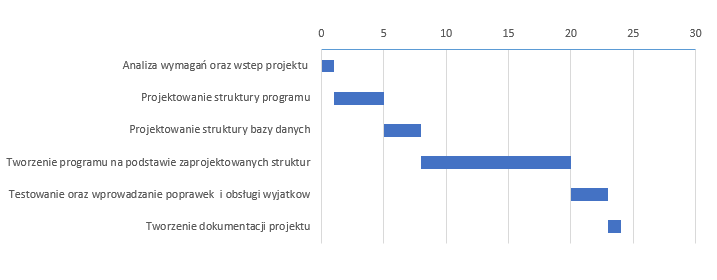
\includegraphics[width=0.8\textwidth]{grafiki/diag_ganta.PNG}
    \caption{\footnotesize Diagram przedstawiający harmonogram działań projektowych \cite{www-2}}
	\label{fig:plotend}
\end{figure}
\newpage
\section{Repozytorium i system kontroli wersji}

\begin{itemize}
    \item Repozytoria: GitHub umożliwia tworzenie repozytoriów, czyli przechowalni, w których można przechowywać pliki projektowe. Repozytoria mogą być publiczne, co oznacza, że są dostępne dla wszystkich, lub prywatne, dostępne tylko dla wybranych użytkowników.
    \item Zarządzanie zmianami: Dzięki systemowi kontroli wersji, takiemu jak Git, programiści mogą śledzić zmiany w kodzie, tworzyć gałęzie do eksperymentowania z nowymi funkcjami lub naprawami błędów, a następnie łączyć te zmiany z główną gałęzią, gdy są gotowe.
    \item Komentarze i dyskusje: Użytkownicy mogą komentować zmiany, zgłaszać problemy i prowadzić dyskusje na temat kodu lub innych plików w repozytorium.
    \item Kontrola dostępu: Właściciele repozytorium mogą kontrolować, kto ma dostęp do repozytorium i jakie uprawnienia mają użytkownicy, na przykład czy mogą zmieniać kod, zgłaszać problemy itp.
\end{itemize}
\subsection*{Github}
Projekt jest umieszczony w repozytorium: 
\newline
\href{https://github.com/DanielKaznowski/w69794_Automat_z_napojami}{\texttt{https://github.com/DanielKaznowski/w69794_Automat_z_napojami}}




% ********** Koniec rozdziału **********
